\subsection{Funkcje Skalarne i Tabelarne}

Zostały stworzone następujące funkcje:
\begin{itemize}
	\item \href{run:Sources/SQL/3. Funkcje Skalarne/017_Utworzenie_funkcji_wyliczajacej_koszt_najmu_obiektu.sql}{\texttt{koszt\_najmu\_obiektu} - Funkcja obliczająca koszt najmu wskazanego obiektu}
	\item \href{run:Sources/SQL/3. Funkcje Skalarne/018_Utworzenie_funkcji_wyliczajacej_koszt_konkretnego_najmu.sql}{\texttt{koszt\_najmu} - Funkcja obliczająca koszt konkretnego najmu}
	\item \href{run:Sources/SQL/3. Funkcje Skalarne/020_Utworzenie_funkcji_wyswietlajacej_adresowke_uzytkownika.sql}{\texttt{adresowka} - Funkcja generująca etykietę adresową dla użytkownika}
	\item \href{run:Sources/SQL/4. Funkcje Tabelarne/021_Utworzenie_funkcji_wyswietlajacej_spozniajacych_sie_uzytkownikow.sql}{\texttt{opoznieni} - Funkcja generująca etykiety dla użytkowników którzy coś wynajęli ale jeszcze nie oddali}
\end{itemize}

\subsubsection{\texttt{koszt\_najmu\_obiektu} - Funkcja obliczająca koszt najmu wskazanego obiektu}

|koszt_najmu_obiektu (@obiekt_id INT, @liczba_dni INT)| - Funkcja ta oblicza koszt najmu obiektu wskazanego w parametrze |@obiekt_id| przez liczbę dni określoną w parametrze |@liczba_dni|, zwracana wartość ma typ |DECIMAL(15, 2)| który jest kompatybilny z typem kolumny \texttt{koszt} w tabeli \texttt{najmy}. Funkcja ta została wydzielona w celu uniknięcia duplikacji kodu w funkcji skalarnej \texttt{koszt\_najmu} z listingu \ref{lst:function-koszt_najmu} oraz w funkcji tabelarnej \texttt{opoznieni} z listingu \ref{lst:function-opoznieni} (strona \pageref{lst:function-opoznieni}).

\begin{lstlisting}[language=SQL, caption={Skrypt tworzący funkcję skalarną \texttt{koszt\_najmu\_obiektu}}, label={lst:function-koszt_najmu_obiektu}]
CREATE FUNCTION koszt_najmu_obiektu (@obiekt_id INT, @liczba_dni INT)
  RETURNS DECIMAL(15, 2)
  AS
  BEGIN
    DECLARE @dzienna_stawka DECIMAL(10,2);

    SELECT @dzienna_stawka = dzienna_stawka_najmu
      FROM obiekty o
      WHERE id = @obiekt_id;

    RETURN @liczba_dni*@dzienna_stawka;
  END
\end{lstlisting}

\subsubsection{\texttt{koszt\_najmu} - Funkcja obliczająca koszt danego najmu}

|koszt_najmu (@najem_id INT)| - Funkcja ta oblicza koszt konkretnego najmu wskazanego w parametrze |@najem_id|, zwracana wartość ma taki sam typ jak funkcja \texttt{koszt\_najmu\_obiektu} która jest wywoływana - czyli |DECIMAL(15, 2)| który jest kompatybilny z typem kolumny \texttt{koszt} w tabeli \texttt{najmy}. Przykład wykorzystania tej funkcji jest w triggerze z listingu \ref{lst:trigger-wylicz_koszt_najmu} (strona \pageref{lst:trigger-wylicz_koszt_najmu}).

\begin{lstlisting}[language=SQL, caption={Skrypt tworzący funkcję skalarną \texttt{koszt\_najmu}}, label={lst:function-koszt_najmu}]
CREATE FUNCTION koszt_najmu (@najem_id INT)
  RETURNS DECIMAL(15, 2)
  AS
  BEGIN
    DECLARE @koszt DECIMAL(15, 2);
    DECLARE @liczba_dni INT;
    DECLARE @obiekt_id INT;
    DECLARE @data_rozpoczecia DATE;
    DECLARE @data_zakonczenia DATE;

    SELECT @data_rozpoczecia = n.data_rozpoczecia,
           @data_zakonczenia = n.data_zakonczenia,
           @obiekt_id = o.id
      FROM najmy n
      JOIN obiekty o on n.obiekt_id = o.id
      WHERE n.id = @najem_id;

    IF @data_zakonczenia IS NULL
      RETURN NULL;

    SELECT @liczba_dni = (1+DATEDIFF(DAY, @data_rozpoczecia, @data_zakonczenia));

    SELECT @koszt = dbo.koszt_najmu_obiektu(@obiekt_id, @liczba_dni);

    RETURN @koszt;
  END
\end{lstlisting}

\subsubsection{\texttt{adresowka} - Funkcja generująca etykietę adresową dla użytkownika}

|adresowka (@uzytkownik_id INT)| - Funkcja ta generuje zawartość etykiety adresowej dla użytkownika wskazanego w parametrze |@uzytkownik_id|, zwracana wartość ma typ |VARCHAR(333)|\footnote{Rozmiar pola bierze się z sumy długości użytych pól (\texttt{nazwisko} i \texttt{imie} po 75 znaków, \texttt{telefon} 30 znaków,\texttt{adres} 150 znaków) oraz znaków dodanych (jedna spacja i dwa znaki nowej lini - \texttt{CHAR(13)}) - jest to najdłuższy możliwy wynik tej funkcji.}. Przykład wykorzystania tej funkcji jest w funkcji tabelarnej z listingu \ref{lst:function-opoznieni}.

\begin{lstlisting}[language=SQL, caption={Skrypt tworzący funkcję skalarną \texttt{adresowka}}, label={lst:function-adresowka}]
CREATE FUNCTION adresowka (@uzytkownik_id INT)
  RETURNS VARCHAR(333) -- 75+75+150+30+3 = 333 - suma długości łączonych pól
  AS
  BEGIN
    DECLARE @adresowka VARCHAR(330);

    SELECT @adresowka = nazwisko + ' ' + imie + CHAR(13) + telefon + CHAR(13) + adres
      FROM uzytkownicy
      WHERE id = @uzytkownik_id;

    RETURN @adresowka;
  END
\end{lstlisting}

\subsubsection{\texttt{opoznieni} - Funkcja generująca etykiety dla użytkowników którzy coś wynajęli ale jeszcze nie oddali}

|opoznieni (@liczba_dni INT)| - Funkcja ta generuje listę obiektów wraz z najemcami, które zostały wynajęte co najmniej liczbę dni wcześniej określoną parametrem |@liczba_dni|. Funkcja ta zwraca tabelę składającą się z identyfikatora najmu, nazwy wynajętego obiektu, liczby dni od rozpoczęcia najmu, szacunkowego kosztu tego najmu na dzień bieżący oraz etykiety adresowej do najemcy.

\begin{figure}[h]
	\centering
    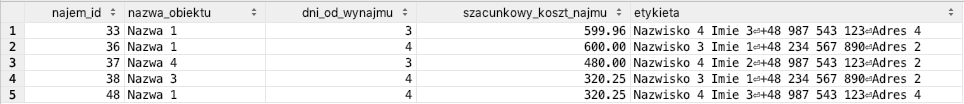
\includegraphics[width=0.8\textwidth]{opoznieni}
	\caption{Uruchomiona funkcja \texttt{opoznieni} z parametrem \texttt{@liczba\_dni} równym 3}
	\label{fig:opoznieni}
\end{figure}

\begin{lstlisting}[language=SQL, caption={Skrypt tworzący funkcję tabelarną \texttt{opoznieni}}, label={lst:function-opoznieni}]
CREATE FUNCTION opoznieni (@liczba_dni INT)
  RETURNS TABLE
  AS
    RETURN (
      SELECT n.id najem_id,
             o.nazwa nazwa_obiektu,
             DATEDIFF(DAY, n.data_rozpoczecia, getdate()) dni_od_wynajmu,
             dbo.koszt_najmu_obiektu(o.id, DATEDIFF(DAY, n.data_rozpoczecia, getdate()) + 1) szacunkowy_koszt_najmu,
             dbo.adresowka(u.id) etykieta
        FROM najmy n
        JOIN obiekty o on n.obiekt_id = o.id
        JOIN uzytkownicy u on n.uzytkownik_id = u.id
        WHERE DATEDIFF(DAY, n.data_rozpoczecia, getdate()) >= @liczba_dni
              AND n.data_zakonczenia IS NULL
    )
\end{lstlisting}